\section{Threshold Sensitivity Protocol}
\label{app:sensitivity}
Threshold sensitivity analysis is implemented in the released artifact as an optional robustness check. The present manuscript does not use threshold-sensitivity results as primary evidence because the main diagnostic conclusions are based on the pre-registered KC-frequency thresholds used in Tables 5, 6, 9, and 10. The artifact evaluates three alternative threshold configurations: (i) an aggressive setting with thresholds \{10, 50, 250\} training interactions, (ii) a conservative setting with thresholds \{30, 150, 750\} training interactions, and (iii) a dynamic quantile-based bucketing scheme where buckets are defined by equal-quantile KCs. These checks are intended to help future users evaluate whether their conclusions are sensitive to the chosen KC-frequency thresholds.

\FloatBarrier

\section{Overall and Bucket-level Performance under Temporal Splits}
\label{app:temporal_performance}
In this section, we present the detailed overall performance (Table~\ref{tab:temporal_overall}) and strata-specific performance breakdowns (Table~\ref{tab:temporal_strata}) under the time-partitioned (temporal) split mode. As shown, deep learning baselines undergo noticeable predictive decay compared to their population-level learner-based counterparts, highlighting the increased difficulty of curriculum-level forecasting. Calibration degradation under temporal splits is reported separately in Appendix~\ref{app:calibration_performance}, Table~\ref{tab:calibration_temporal}.

\input{tables/table_07_overall_performance_temporal}
\input{tables/table_08_kc_strata_performance_temporal}

\clearpage
\section{Detailed Calibration Results}
\label{app:calibration_performance}
Detailed calibration results by frequency stratum for the learner-based split are reported in Table~\ref{tab:calibration_learner}. The corresponding temporal calibration breakdowns, computed after the label-alignment correction documented in Appendix~\ref{app:alignment} and used as the numerical basis for Figure~\ref{fig:reliability_junyi_temporal}, are reported in Table~\ref{tab:calibration_temporal}.

\begin{table*}[htbp]
\caption{Calibration Breakdown by Frequency Stratum}
\label{tab:calibration_learner}
\centering
\resizebox{\textwidth}{!}{%
\begin{tabular}{lllrcccccc}
\toprule
Dataset & Model & Bucket & Rel. & \#Events & ECE & Brier & UNC & REL & RES \\
\midrule
ASSISTments 2012 & IRT & dense & R & 523,971 & $0.0031 \pm 0.0006$ & $0.2103 \pm 0.0003$ & $0.2103$ & $0.0000$ & $0.0000$ \\
 &  & medium & R & 5,963 & $0.1598 \pm 0.0190$ & $0.2742 \pm 0.0075$ & $0.2484$ & $0.0258$ & $0.0000$ \\
 &  & sparse & L & 415 & $0.0777 \pm 0.0555$ & $0.2420 \pm 0.0218$ & $0.2337$ & $0.0084$ & $0.0000$ \\
 &  & Very Sparse & I & 16 & $0.2244 \pm 0.0666$ & $0.2996 \pm 0.0261$ & $0.2459$ & $0.0537$ & $0.0000$ \\
 &  & Strict Cold-start & I & 4 & $0.6962$ & $0.4848$ & $0.0000$ & $0.4848$ & $0.0000$ \\
 & DKT & dense & R & 523,971 & $0.0602 \pm 0.0022$ & $0.1931 \pm 0.0010$ & $0.2103$ & $0.0053$ & $0.0223$ \\
 &  & medium & R & 5,963 & $0.1621 \pm 0.0256$ & $0.2297 \pm 0.0144$ & $0.2484$ & $0.0301$ & $0.0479$ \\
 &  & sparse & L & 415 & $0.2333 \pm 0.0084$ & $0.2502 \pm 0.0098$ & $0.2337$ & $0.0624$ & $0.0451$ \\
 &  & Very Sparse & I & 16 & $0.1782 \pm 0.0666$ & $0.1464 \pm 0.0786$ & $0.2459$ & $0.0862$ & $0.1849$ \\
 &  & Strict Cold-start & I & 4 & $0.5014$ & $0.2540$ & $0.0000$ & $0.2539$ & $0.0000$ \\
 & SimpleKT & dense & R & 523,971 & $0.1136 \pm 0.0066$ & $0.2116 \pm 0.0019$ & $0.2103$ & $0.0201$ & $0.0186$ \\
 &  & medium & R & 5,963 & $0.1541 \pm 0.0051$ & $0.2272 \pm 0.0086$ & $0.2484$ & $0.0273$ & $0.0478$ \\
 &  & sparse & L & 415 & $0.2280 \pm 0.0197$ & $0.2525 \pm 0.0116$ & $0.2337$ & $0.0594$ & $0.0392$ \\
 &  & Very Sparse & I & 16 & $0.2451 \pm 0.0511$ & $0.2165 \pm 0.0461$ & $0.2459$ & $0.0852$ & $0.1148$ \\
 &  & Strict Cold-start & I & 4 & $0.5224$ & $0.2761$ & $0.0000$ & $0.2758$ & $0.0000$ \\
\midrule
Junyi Academy & IRT & dense & R & 3,226,541 & $0.0026 \pm 0.0018$ & $0.2078 \pm 0.0007$ & $0.2078$ & $0.0000$ & $0.0000$ \\
 &  & medium & R & 3,706 & $0.1209 \pm 0.0082$ & $0.2579 \pm 0.0033$ & $0.2432$ & $0.0147$ & $0.0000$ \\
 & DKT & dense & R & 3,226,541 & $0.0389 \pm 0.0022$ & $0.1804 \pm 0.0008$ & $0.2078$ & $0.0022$ & $0.0294$ \\
 &  & medium & R & 3,706 & $0.2513 \pm 0.0217$ & $0.3077 \pm 0.0144$ & $0.2432$ & $0.0741$ & $0.0091$ \\
 & SimpleKT & dense & R & 3,232,614 & $0.0792 \pm 0.0051$ & $0.1884 \pm 0.0020$ & $0.2079$ & $0.0084$ & $0.0279$ \\
 &  & medium & R & 3,836 & $0.1073 \pm 0.0156$ & $0.2307 \pm 0.0103$ & $0.2417$ & $0.0149$ & $0.0260$ \\
\midrule
XES3G5M & IRT & dense & R & 1,269,345 & $0.1546 \pm 0.0033$ & $0.1861 \pm 0.0008$ & $0.1622$ & $0.0239$ & $0.0000$ \\
 &  & medium & R & 12,889 & $0.1421 \pm 0.0060$ & $0.1897 \pm 0.0015$ & $0.1695$ & $0.0202$ & $0.0000$ \\
 &  & sparse & R & 1,969 & $0.1119 \pm 0.0096$ & $0.1982 \pm 0.0026$ & $0.1856$ & $0.0126$ & $0.0000$ \\
 &  & Very Sparse & L & 114 & $0.0850 \pm 0.0420$ & $0.2059 \pm 0.0118$ & $0.1973$ & $0.0085$ & $0.0000$ \\
 &  & Strict Cold-start & I & 5 & $0.2362 \pm 0.1144$ & $0.2269 \pm 0.0836$ & $0.1613$ & $0.0656$ & $0.0000$ \\
 & DKT & dense & R & 1,268,696 & $0.0388 \pm 0.0023$ & $0.1221 \pm 0.0021$ & $0.1614$ & $0.0027$ & $0.0415$ \\
 &  & medium & R & 12,980 & $0.0906 \pm 0.0172$ & $0.1231 \pm 0.0099$ & $0.1681$ & $0.0133$ & $0.0571$ \\
 &  & sparse & R & 2,010 & $0.1187 \pm 0.0154$ & $0.1412 \pm 0.0087$ & $0.1864$ & $0.0195$ & $0.0637$ \\
 &  & Very Sparse & L & 112 & $0.1840 \pm 0.0372$ & $0.1806 \pm 0.0364$ & $0.2048$ & $0.0542$ & $0.0762$ \\
 &  & Strict Cold-start & I & 4 & $0.4472 \pm 0.0937$ & $0.2655 \pm 0.0391$ & $0.1022$ & $0.2217$ & $0.0583$ \\
 & SimpleKT & dense & R & 1,268,696 & $0.1145 \pm 0.0011$ & $0.1547 \pm 0.0029$ & $0.1614$ & $0.0179$ & $0.0237$ \\
 &  & medium & R & 12,980 & $0.1114 \pm 0.0076$ & $0.1351 \pm 0.0060$ & $0.1681$ & $0.0169$ & $0.0488$ \\
 &  & sparse & R & 2,010 & $0.1248 \pm 0.0085$ & $0.1477 \pm 0.0050$ & $0.1864$ & $0.0215$ & $0.0593$ \\
 &  & Very Sparse & L & 112 & $0.1832 \pm 0.0111$ & $0.1727 \pm 0.0110$ & $0.2048$ & $0.0538$ & $0.0850$ \\
 &  & Strict Cold-start & I & 4 & $0.5738 \pm 0.2468$ & $0.4192 \pm 0.2186$ & $0.1022$ & $0.3844$ & $0.0661$ \\
\bottomrule

\end{tabular}%
}

\vspace{1ex}
{\scriptsize \textbf{Note:} Reliability flags (R/L/I) follow Section 3.5. Mean $\pm$ standard deviation and event counts are over four unique learner-based partitions (seeds 2025 and 2026 averaged first). IRT shows low ECE in several learner-based cohorts, but $\text{RES} = 0$ across strata indicates base-rate-like behavior with no resolving power (Section 4.2); IRT calibration should therefore be interpreted jointly with AUC and Brier resolution.\par}

\end{table*}

\input{tables/table_10_calibration_breakdown_temporal}
\clearpage

\section{Diagnostic Interpretation Guide}
\label{app:interpretation}
To assist researchers and practitioners in applying our diagnostic protocol, we provide Table~\ref{tab:interpretation_guide} which maps common empirical diagnostic patterns observed during evaluation to their theoretical and operational educational interpretation.

\input{tables/table_11_diagnostic_interpretation_guide}

\section{Dataset Conditions for Sparse-KC Calibration Vulnerability}
\label{app:dataset_conditions}
Table~\ref{tab:a5_dataset_conditions} accompanies Section~\ref{sec:a5_dataset_dependent}. It reports only quantities that can be computed from training-fold frequencies, training-only KC covariates, and the event-level ECE already published in Table~\ref{tab:calibration_learner}.

\begin{table*}[htbp]
\caption{Dataset conditions associated with observable sparse-KC calibration vulnerability. All six rows are structural or metric observations computed from training-fold frequencies and published event-level SimpleKT ECE (Table~\ref{tab:calibration_learner}); they are FINDINGS, not causal claims. Hierarchical curriculum, ceiling effects, item-feature richness, and tagging granularity are \emph{not} listed here because they are untested (HYPOTHESIS; see text). Sparse mass is the share of KCs with $f_{\mathrm{train}}<100$ (sparse + very sparse + strict). Test support uses the protocol reliability flags (R/L/I). Coupling is Spearman $\rho$ between $\log(1+f_{\mathrm{train}})$ and the named training-only covariate.}
\label{tab:a5_dataset_conditions}
\centering
\footnotesize
\setlength{\tabcolsep}{3.5pt}
\begin{tabularx}{\textwidth}{>{\raggedright\arraybackslash}p{3.3cm}XXX}
\toprule
\textbf{Condition} & \textbf{ASSISTments 2012} & \textbf{Junyi Academy} & \textbf{XES3G5M} \\
\midrule
Meaningful sparse mass & Present (18.9\% of KCs) & Absent (0.0\% of KCs) & Present (22.5\% of KCs) \\
\midrule
Sufficient test support & Partial (sparse $N=415$ L; very-sparse $N=16$ I) & Absent (0 sparse/very-sparse test events) & Present (sparse $N=2{,}010$ R; very-sparse $N=112$ L) \\
\midrule
Frequency--difficulty coupling & Present, expected dir.\ ($\rho=-0.227$; sparse harder) & Present, expected dir.\ ($\rho=-0.416$; sparse harder) & Weak, opposite-signed ($\rho=+0.087$) \\
\midrule
Curriculum-position coupling & Present ($\rho=-0.308$) & Present ($\rho=-0.324$) & Weak ($\rho=-0.125$) \\
\midrule
Item-support imbalance & High (dense 205.0 vs sparse 1.0 items/KC) & Median 18.0 items/KC (no sparse contrast) & High (dense 9.0 vs sparse 1.0 items/KC) \\
\midrule
Observed calibration gradient (SimpleKT, event-level) & Monotonic increase ($0.114\to 0.154\to 0.228$) & Dense$\to$medium only ($\Delta$ECE$=+0.028$); sparse empty & Flat dense$\to$sparse ($0.114\to 0.111\to 0.125$) \\
\bottomrule
\end{tabularx}

\vspace{1ex}
{\scriptsize \textbf{Note:} Event-level ECE matches Table~\ref{tab:calibration_learner}. XES3G5M IRT ECE \emph{decreases} from dense to sparse (inverted), whereas DKT increases; the SimpleKT row is therefore not a dataset-universal gradient. Junyi temporal splits do populate sparse strata (see Table~\ref{tab:temporal_strata}), so the learner-based empty-sparse pattern is threshold- and volume-dependent.\par}
\end{table*}


\section{When Sparse-Concept Diagnostics Are Informative}
\label{app:a8_need}
Tables~\ref{tab:a8_need_framework} and~\ref{tab:a8_dataset_need} accompany Section~\ref{sec:a8_when_needed}. Need levels reuse the protocol's pre-registered sparse threshold and reliability flags; C4 is qualitative intended use.

\input{tables/table_14_need_framework}
\input{tables/table_15_dataset_need}

\section{Controlled Sparsification of Training Evidence}
\label{app:a9_sparsify}
The selection rule was recorded before reduced-evidence ECE was inspected (\path{controlled_sparsification_protocol.md}).
On each dataset, eligible KCs had $f_{\mathrm{train}}\ge 500$, $N_{\mathrm{test}}\ge 100$, and at least 20 positive and 20 negative test labels.
If more than 30 KCs qualified, ten were taken from each tertile of the training-only difficulty proxy $1-\bar{c}_{\mathrm{train}}$, sorted by \texttt{kc\_id}.
ECE was not a selection criterion.

Training rows of selected KCs were downsampled to 500, 100, or 50 interactions with a deterministic RNG; validation, test, KC identifiers, and non-selected training rows were unchanged.
Official processed \path{train.csv} files were not overwritten.
DKT and SimpleKT were retrained on ASSISTments 2012, Junyi Academy, and XES3G5M, learner-based fold 0, seed 42.
The 100\% control is the published prediction export for that seed, not a second A9 retrain of the full fold.

Primary outcomes are within-KC $\Delta$ECE and $\Delta$REL (Table~\ref{tab:a9_sparsification}, Figure~\ref{fig:a9_sparsify}).
A within-KC ECE increase after reducing training rows is not universal: it is absent on ASSISTments 2012, large for SimpleKT on Junyi Academy, and modest for SimpleKT on XES3G5M.
We do not claim that real-world sparsity always causes miscalibration.

\begin{table}[htbp]
\caption{Controlled sparsification: within-KC change in primary calibration outcomes on the held-out test events of 30 originally dense KCs per dataset (seed 42). $\Delta = $ reduced $-$ published full. Positive values mean worse calibration after reducing training rows for the same KC. 95\% CIs are bootstrap over KCs. This is a validation experiment; it does not claim that real-world sparsity always causes miscalibration.}
\label{tab:a9_sparsification}
\centering
\scriptsize
\begin{tabular}{llcccc}
\toprule
Dataset & Model & Rows kept & $\Delta$ECE [95\% CI] & $\Delta$REL [95\% CI] & Share ECE$\uparrow$ \\
\midrule
ASSISTments 2012 & DKT & 500 & $-0.047$ [$-0.060$, $-0.033$] & $-0.015$ [$-0.022$, $-0.010$] & 10\% \\
ASSISTments 2012 & DKT & 100 & $-0.024$ [$-0.046$, $-0.001$] & $-0.008$ [$-0.017$, $0.001$] & 30\% \\
ASSISTments 2012 & DKT & 50 & $-0.017$ [$-0.034$, $0.002$] & $-0.008$ [$-0.016$, $-0.002$] & 43\% \\
ASSISTments 2012 & SimpleKT & 500 & $-0.026$ [$-0.047$, $-0.002$] & $-0.008$ [$-0.017$, $0.003$] & 20\% \\
ASSISTments 2012 & SimpleKT & 100 & $0.002$ [$-0.023$, $0.029$] & $0.000$ [$-0.013$, $0.014$] & 43\% \\
ASSISTments 2012 & SimpleKT & 50 & $0.002$ [$-0.021$, $0.025$] & $0.001$ [$-0.011$, $0.012$] & 47\% \\
\midrule
Junyi Academy & DKT & 500 & $-0.021$ [$-0.041$, $-0.001$] & $-0.007$ [$-0.013$, $-0.002$] & 30\% \\
Junyi Academy & DKT & 100 & $-0.010$ [$-0.031$, $0.011$] & $-0.003$ [$-0.009$, $0.002$] & 37\% \\
Junyi Academy & DKT & 50 & $-0.004$ [$-0.022$, $0.013$] & $-0.002$ [$-0.008$, $0.003$] & 57\% \\
Junyi Academy & SimpleKT & 500 & $0.101$ [$0.081$, $0.120$] & $0.048$ [$0.035$, $0.060$] & 93\% \\
Junyi Academy & SimpleKT & 100 & $0.132$ [$0.109$, $0.155$] & $0.061$ [$0.047$, $0.077$] & 100\% \\
Junyi Academy & SimpleKT & 50 & $0.135$ [$0.110$, $0.161$] & $0.061$ [$0.047$, $0.074$] & 100\% \\
\midrule
XES3G5M & DKT & 500 & $-0.008$ [$-0.019$, $0.004$] & $-0.002$ [$-0.005$, $0.001$] & 27\% \\
XES3G5M & DKT & 100 & $0.001$ [$-0.009$, $0.011$] & $-0.001$ [$-0.004$, $0.002$] & 47\% \\
XES3G5M & DKT & 50 & $0.018$ [$0.006$, $0.029$] & $0.003$ [$0.000$, $0.006$] & 77\% \\
XES3G5M & SimpleKT & 500 & $0.014$ [$-0.002$, $0.032$] & $0.011$ [$0.001$, $0.023$] & 57\% \\
XES3G5M & SimpleKT & 100 & $0.015$ [$0.002$, $0.030$] & $0.007$ [$0.001$, $0.013$] & 63\% \\
XES3G5M & SimpleKT & 50 & $0.032$ [$0.021$, $0.043$] & $0.018$ [$0.012$, $0.025$] & 90\% \\
\bottomrule
\end{tabular}
\end{table}


\begin{figure}[htbp]
\centering
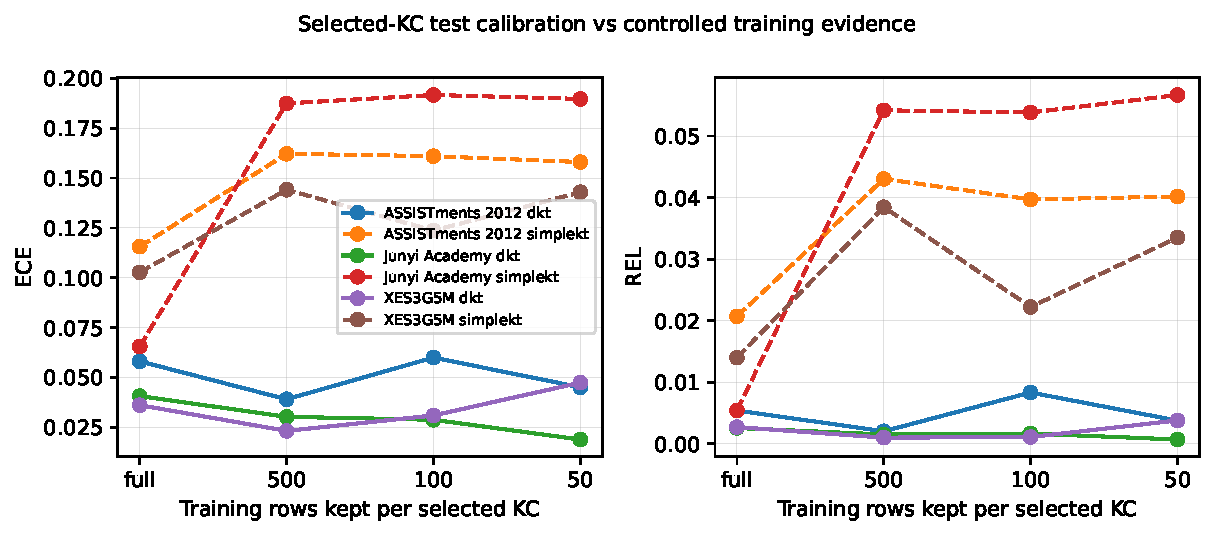
\includegraphics[width=0.85\linewidth]{figures/a9_ece_rel_vs_evidence.pdf}
\caption{Selected-KC test ECE and REL versus training rows kept per selected KC on ASSISTments 2012, Junyi Academy, and XES3G5M (seed 42). The full points are the published models. This figure is descriptive; inference uses the paired within-KC bootstrap in Table~\ref{tab:a9_sparsification}.}
\label{fig:a9_sparsify}
\end{figure}

\section[Bayesian Knowledge Tracing Numerical Instability and Transition]{Bayesian Knowledge Tracing Numerical Instability and Transition}
\label{app:bkt_instability}
During our initial protocol implementation, we instantiated Bayesian Knowledge Tracing (BKT) as the classical baseline utilizing the popular \texttt{pyBKT} library (v1.4.1). However, on all three large-scale datasets, BKT suffered from severe numerical instability during EM parameter estimation. Specifically, for sparse and very sparse concept strata, the scarcity of interaction logs triggered a divide-by-zero error in the M-step update equation for the prior parameter, resulting in \texttt{NaN} value assignments. Consequently, the model's predictions degenerated into deterministic binary outputs ($p_{pred} \in \{0.0, \text{NaN}\}$), yielding a flat $0.50$ AUC and extreme NLL values ranging between $23.7$ and $28.0$. To maintain scientific integrity and standard baseline comparison, we transitioned to Item Response Theory (IRT 1PL / Rasch Model) as the primary classical baseline. The raw prediction CSV files for the failed BKT runs are preserved within the codebase predictions directory for transparency.

\section{Prediction--Label Alignment Audit for Temporal Splits}
\label{app:alignment}
During the temporal-split audit, we identified a prediction--label alignment issue in the temporal evaluation pipeline. The issue occurred when exported model predictions were matched back to temporal test instances after sequence construction and cohort filtering. In the affected code path, an alignment discrepancy in the temporal evaluation pipeline made some exported $p_{pred}$ values correspond to incorrect $y_{true}$ entries.

The main symptom was not limited to strict cold-start KCs. Deep KT baselines produced near-random AUC even on warm temporal cohorts, where KCs had sufficient training-fold evidence. This behavior was a red flag because a static IRT baseline still achieved meaningful AUC on the same warm cohorts, whereas DKT and SimpleKT collapsed to approximately random ranking.

We detected the issue using two sanity checks. First, we compared warm-cohort AUC against the IRT reference baseline; near-random deep KT AUC on warm KCs was treated as an alignment warning rather than as evidence of genuine temporal generalization failure. Second, we computed prediction--label correlation on warm-cohort slices and verified whether $\mathbb{E}[p_{pred}\mid y=1]$ exceeded $\mathbb{E}[p_{pred}\mid y=0]$. The correction preserves a stable test-instance identity through temporal splitting, sequence construction, prediction export, cohort filtering, and metric computation. Metrics are computed only after pairing predictions and labels by this stable identity rather than by transient row position.

After applying the correction consistently across datasets, warm-cohort AUC for the affected deep KT baselines recovered above the sanity threshold, and prediction--label correlations became positive. These checks were then used before re-running the temporal diagnostics reported in the paper. This audit reinforces the central message of the protocol: temporal cold-start results should be accompanied by warm-cohort and prediction--label sanity checks to distinguish genuine concept-level cold-start difficulty from alignment artifacts.

\clearpage
\section{Controlled Fault Injection for Predictive-Sanity Validation}
\label{app:l8_fault}
The alignment case in Appendix~\ref{app:alignment} is one observed defect. A single catch does not by itself establish how L8 behaves under other alignment failures. This section reports a \emph{validation experiment}---not a pre-registered primary analysis---that injects controlled faults into \emph{in-memory copies} of the existing temporal prediction CSVs (DKT and SimpleKT, seed 42, three datasets). The original prediction files are never overwritten.

\paragraph{Fault classes.}
F1 and F2 pair $p_t$ with $y_{t+1}$ and $y_{t-1}$ within each learner. F3 shifts $p_{\mathrm{pred}}$ by one timestep within learner. F4 shuffles predictions within learner. F5 reassigns $p_{\mathrm{pred}}$ by row index after a different sort (a global position mismatch of the class that motivated the original L8 catch). F6 swaps a random $1\%$, $5\%$, $10\%$, $25\%$, or $50\%$ of rows.

\paragraph{Detection signals and rule.}
L8 records warm-cohort AUC, $\mathrm{corr}(p_{\mathrm{pred}},y)$, $\mathbb{E}[p_{\mathrm{pred}}\mid y=1]-\mathbb{E}[p_{\mathrm{pred}}\mid y=0]$, the fraction of missing or unmatched stable ids, and prediction--label identity consistency against the official temporal test split. A file is flagged if any of the following hold: warm AUC $< 0.55$; warm AUC more than $0.05$ below the clean IRT warm-cohort reference; non-positive correlation or conditional-mean gap; or an identity-mismatch rate more than $1$ percentage point above that same file's clean-pipeline identity-mismatch rate. The last clause uses the correct pipeline as the reference distribution: Junyi Academy has a small baseline identity collision ($\approx 0.9\%$) from duplicate stable ids, so an absolute zero-tolerance cutoff would false-positive the clean export. Thresholds were not chosen after inspecting the injected-fault outcomes.

\paragraph{Results.}
Table~\ref{tab:l8_fault_injection} reports detection rates over six files (two models $\times$ three datasets). The clean copies produced $0/6$ false positives. L8 detected all F1, F2, and F5 injections ($6/6$ each). F1 and F2 were caught by the identity check: adjacent-label shifts left warm AUC in the $0.60$--$0.81$ range because learner sequences are autocorrelated. F5---the row-index mismatch class---collapsed warm AUC to $\approx 0.50$ and fired the original Appendix~\ref{app:alignment} signals. F3 was never detected ($0/6$): shifting $p_{\mathrm{pred}}$ by one step does not change exported labels or ids, and residual association remains positive. F4 was detected on $2/6$ files (XES3G5M only, via collapse versus IRT). F6 was undetected at corruption rates $\le 25\%$ and reached $3/6$ at $50\%$ (Figure~\ref{fig:l8_fault_curve}). Overall detection was $23/60$ injected faults ($38.3\%$).

L8 is therefore sensitive to the identity-shifted-label and global row-index-mismatch classes tested here, and only weakly sensitive to within-learner shuffles and high-rate partial swaps. It is \emph{not} sensitive to adjacent-timestep prediction shifts that preserve autocorrelation. We do not claim that L8 detects every evaluation bug.

\begin{table}[htbp]
\caption{Controlled fault-injection validation of channel L8 (temporal warm cohort). This is a validation experiment, not a pre-registered primary analysis. Detection uses the Appendix~\ref{app:alignment} signals plus identity consistency against official test-split labels on a stable instance id: warm AUC $< 0.55$, or warm AUC more than $0.05$ below the clean IRT warm-cohort reference, or non-positive $\mathrm{corr}(p,y)$ / conditional-mean gap, or exported $y$ elevated more than $1$ percentage point above the same file's clean-pipeline identity-mismatch rate. Thresholds were not tuned on the injected faults. L8 is sensitive to some of the tested alignment-fault classes; it is not claimed to detect all bugs.}\label{tab:l8_fault_injection}
\centering
\small
\begin{tabular}{lc}
\toprule
\textbf{Condition} & \textbf{Detection rate} \\
\midrule
Clean pipeline (false-positive check) & 0/6 \\
F1 label shift $+1$ & 100\% (6/6) \\
F2 label shift $-1$ & 100\% (6/6) \\
F3 prediction shift & 0\% (0/6) \\
F4 within-learner shuffle & 33\% (2/6) \\
F5 row-index mismatch & 100\% (6/6) \\
\midrule
F6 partial mismatch $1\%$ & 0\% (0/6) \\
F6 partial mismatch $5\%$ & 0\% (0/6) \\
F6 partial mismatch $10\%$ & 0\% (0/6) \\
F6 partial mismatch $25\%$ & 0\% (0/6) \\
F6 partial mismatch $50\%$ & 50\% (3/6) \\
\midrule
All injected faults & 23/60 (38.3\%) \\
\bottomrule
\end{tabular}

\vspace{1ex}
{\scriptsize \textbf{Note:} Counts pool DKT and SimpleKT $\times$ three datasets (six files). Original prediction CSVs are not modified. Adjacent-timestep prediction shifts (F3) often retain warm AUC because learner sequences are autocorrelated; L8 as specified does not treat that residual association as a failure.\par}
\end{table}


\begin{figure}[htbp]
\centering
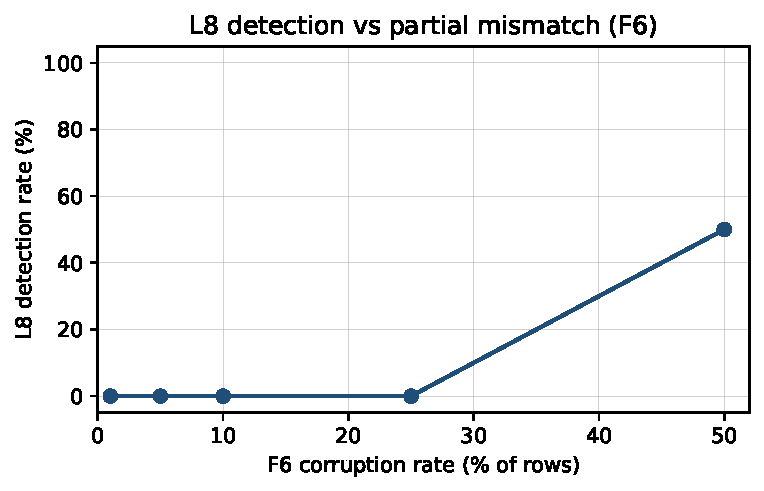
\includegraphics[width=0.72\linewidth]{figures/l8_fault_injection_detection_curve.pdf}
\caption{L8 detection rate versus F6 partial-mismatch corruption, pooled over six temporal prediction files. Detection remains $0$ through $25\%$ and reaches $50\%$ ($3/6$ files) at $50\%$ corruption. This is a validation curve, not a tuned operating characteristic.}
\label{fig:l8_fault_curve}
\end{figure}
